% Options for packages loaded elsewhere
% Options for packages loaded elsewhere
\PassOptionsToPackage{unicode}{hyperref}
\PassOptionsToPackage{hyphens}{url}
\PassOptionsToPackage{dvipsnames,svgnames,x11names}{xcolor}
%
\documentclass[
  letterpaper,
  DIV=11,
  numbers=noendperiod]{scrreprt}
\usepackage{xcolor}
\usepackage{amsmath,amssymb}
\setcounter{secnumdepth}{5}
\usepackage{iftex}
\ifPDFTeX
  \usepackage[T1]{fontenc}
  \usepackage[utf8]{inputenc}
  \usepackage{textcomp} % provide euro and other symbols
\else % if luatex or xetex
  \usepackage{unicode-math} % this also loads fontspec
  \defaultfontfeatures{Scale=MatchLowercase}
  \defaultfontfeatures[\rmfamily]{Ligatures=TeX,Scale=1}
\fi
\usepackage{lmodern}
\ifPDFTeX\else
  % xetex/luatex font selection
\fi
% Use upquote if available, for straight quotes in verbatim environments
\IfFileExists{upquote.sty}{\usepackage{upquote}}{}
\IfFileExists{microtype.sty}{% use microtype if available
  \usepackage[]{microtype}
  \UseMicrotypeSet[protrusion]{basicmath} % disable protrusion for tt fonts
}{}
\makeatletter
\@ifundefined{KOMAClassName}{% if non-KOMA class
  \IfFileExists{parskip.sty}{%
    \usepackage{parskip}
  }{% else
    \setlength{\parindent}{0pt}
    \setlength{\parskip}{6pt plus 2pt minus 1pt}}
}{% if KOMA class
  \KOMAoptions{parskip=half}}
\makeatother
% Make \paragraph and \subparagraph free-standing
\makeatletter
\ifx\paragraph\undefined\else
  \let\oldparagraph\paragraph
  \renewcommand{\paragraph}{
    \@ifstar
      \xxxParagraphStar
      \xxxParagraphNoStar
  }
  \newcommand{\xxxParagraphStar}[1]{\oldparagraph*{#1}\mbox{}}
  \newcommand{\xxxParagraphNoStar}[1]{\oldparagraph{#1}\mbox{}}
\fi
\ifx\subparagraph\undefined\else
  \let\oldsubparagraph\subparagraph
  \renewcommand{\subparagraph}{
    \@ifstar
      \xxxSubParagraphStar
      \xxxSubParagraphNoStar
  }
  \newcommand{\xxxSubParagraphStar}[1]{\oldsubparagraph*{#1}\mbox{}}
  \newcommand{\xxxSubParagraphNoStar}[1]{\oldsubparagraph{#1}\mbox{}}
\fi
\makeatother


\usepackage{longtable,booktabs,array}
\usepackage{calc} % for calculating minipage widths
% Correct order of tables after \paragraph or \subparagraph
\usepackage{etoolbox}
\makeatletter
\patchcmd\longtable{\par}{\if@noskipsec\mbox{}\fi\par}{}{}
\makeatother
% Allow footnotes in longtable head/foot
\IfFileExists{footnotehyper.sty}{\usepackage{footnotehyper}}{\usepackage{footnote}}
\makesavenoteenv{longtable}
\usepackage{graphicx}
\makeatletter
\newsavebox\pandoc@box
\newcommand*\pandocbounded[1]{% scales image to fit in text height/width
  \sbox\pandoc@box{#1}%
  \Gscale@div\@tempa{\textheight}{\dimexpr\ht\pandoc@box+\dp\pandoc@box\relax}%
  \Gscale@div\@tempb{\linewidth}{\wd\pandoc@box}%
  \ifdim\@tempb\p@<\@tempa\p@\let\@tempa\@tempb\fi% select the smaller of both
  \ifdim\@tempa\p@<\p@\scalebox{\@tempa}{\usebox\pandoc@box}%
  \else\usebox{\pandoc@box}%
  \fi%
}
% Set default figure placement to htbp
\def\fps@figure{htbp}
\makeatother





\setlength{\emergencystretch}{3em} % prevent overfull lines

\providecommand{\tightlist}{%
  \setlength{\itemsep}{0pt}\setlength{\parskip}{0pt}}



 


\usepackage{booktabs}
\usepackage{caption}
\usepackage{longtable}
\usepackage{colortbl}
\usepackage{array}
\usepackage{anyfontsize}
\usepackage{multirow}
\KOMAoption{captions}{tableheading}
\makeatletter
\@ifpackageloaded{bookmark}{}{\usepackage{bookmark}}
\makeatother
\makeatletter
\@ifpackageloaded{caption}{}{\usepackage{caption}}
\AtBeginDocument{%
\ifdefined\contentsname
  \renewcommand*\contentsname{Table of contents}
\else
  \newcommand\contentsname{Table of contents}
\fi
\ifdefined\listfigurename
  \renewcommand*\listfigurename{List of Figures}
\else
  \newcommand\listfigurename{List of Figures}
\fi
\ifdefined\listtablename
  \renewcommand*\listtablename{List of Tables}
\else
  \newcommand\listtablename{List of Tables}
\fi
\ifdefined\figurename
  \renewcommand*\figurename{Figure}
\else
  \newcommand\figurename{Figure}
\fi
\ifdefined\tablename
  \renewcommand*\tablename{Table}
\else
  \newcommand\tablename{Table}
\fi
}
\@ifpackageloaded{float}{}{\usepackage{float}}
\floatstyle{ruled}
\@ifundefined{c@chapter}{\newfloat{codelisting}{h}{lop}}{\newfloat{codelisting}{h}{lop}[chapter]}
\floatname{codelisting}{Listing}
\newcommand*\listoflistings{\listof{codelisting}{List of Listings}}
\makeatother
\makeatletter
\makeatother
\makeatletter
\@ifpackageloaded{caption}{}{\usepackage{caption}}
\@ifpackageloaded{subcaption}{}{\usepackage{subcaption}}
\makeatother
\usepackage{bookmark}
\IfFileExists{xurl.sty}{\usepackage{xurl}}{} % add URL line breaks if available
\urlstyle{same}
\hypersetup{
  pdftitle={Autonomous Vehicle Industry Strategy \& Analysis},
  pdfauthor={Ronak Shah},
  colorlinks=true,
  linkcolor={blue},
  filecolor={Maroon},
  citecolor={Blue},
  urlcolor={Blue},
  pdfcreator={LaTeX via pandoc}}


\title{Autonomous Vehicle Industry Strategy \& Analysis}
\usepackage{etoolbox}
\makeatletter
\providecommand{\subtitle}[1]{% add subtitle to \maketitle
  \apptocmd{\@title}{\par {\large #1 \par}}{}{}
}
\makeatother
\subtitle{An In-depth Look at Autonomous Vehicle Consumer \& Industry
Report}
\author{Ronak Shah}
\date{2025-11-27}
\begin{document}
\maketitle

\renewcommand*\contentsname{Table of contents}
{
\hypersetup{linkcolor=}
\setcounter{tocdepth}{2}
\tableofcontents
}

\bookmarksetup{startatroot}

\chapter*{Preface}\label{preface}
\addcontentsline{toc}{chapter}{Preface}

\markboth{Preface}{Preface}

\begin{center}
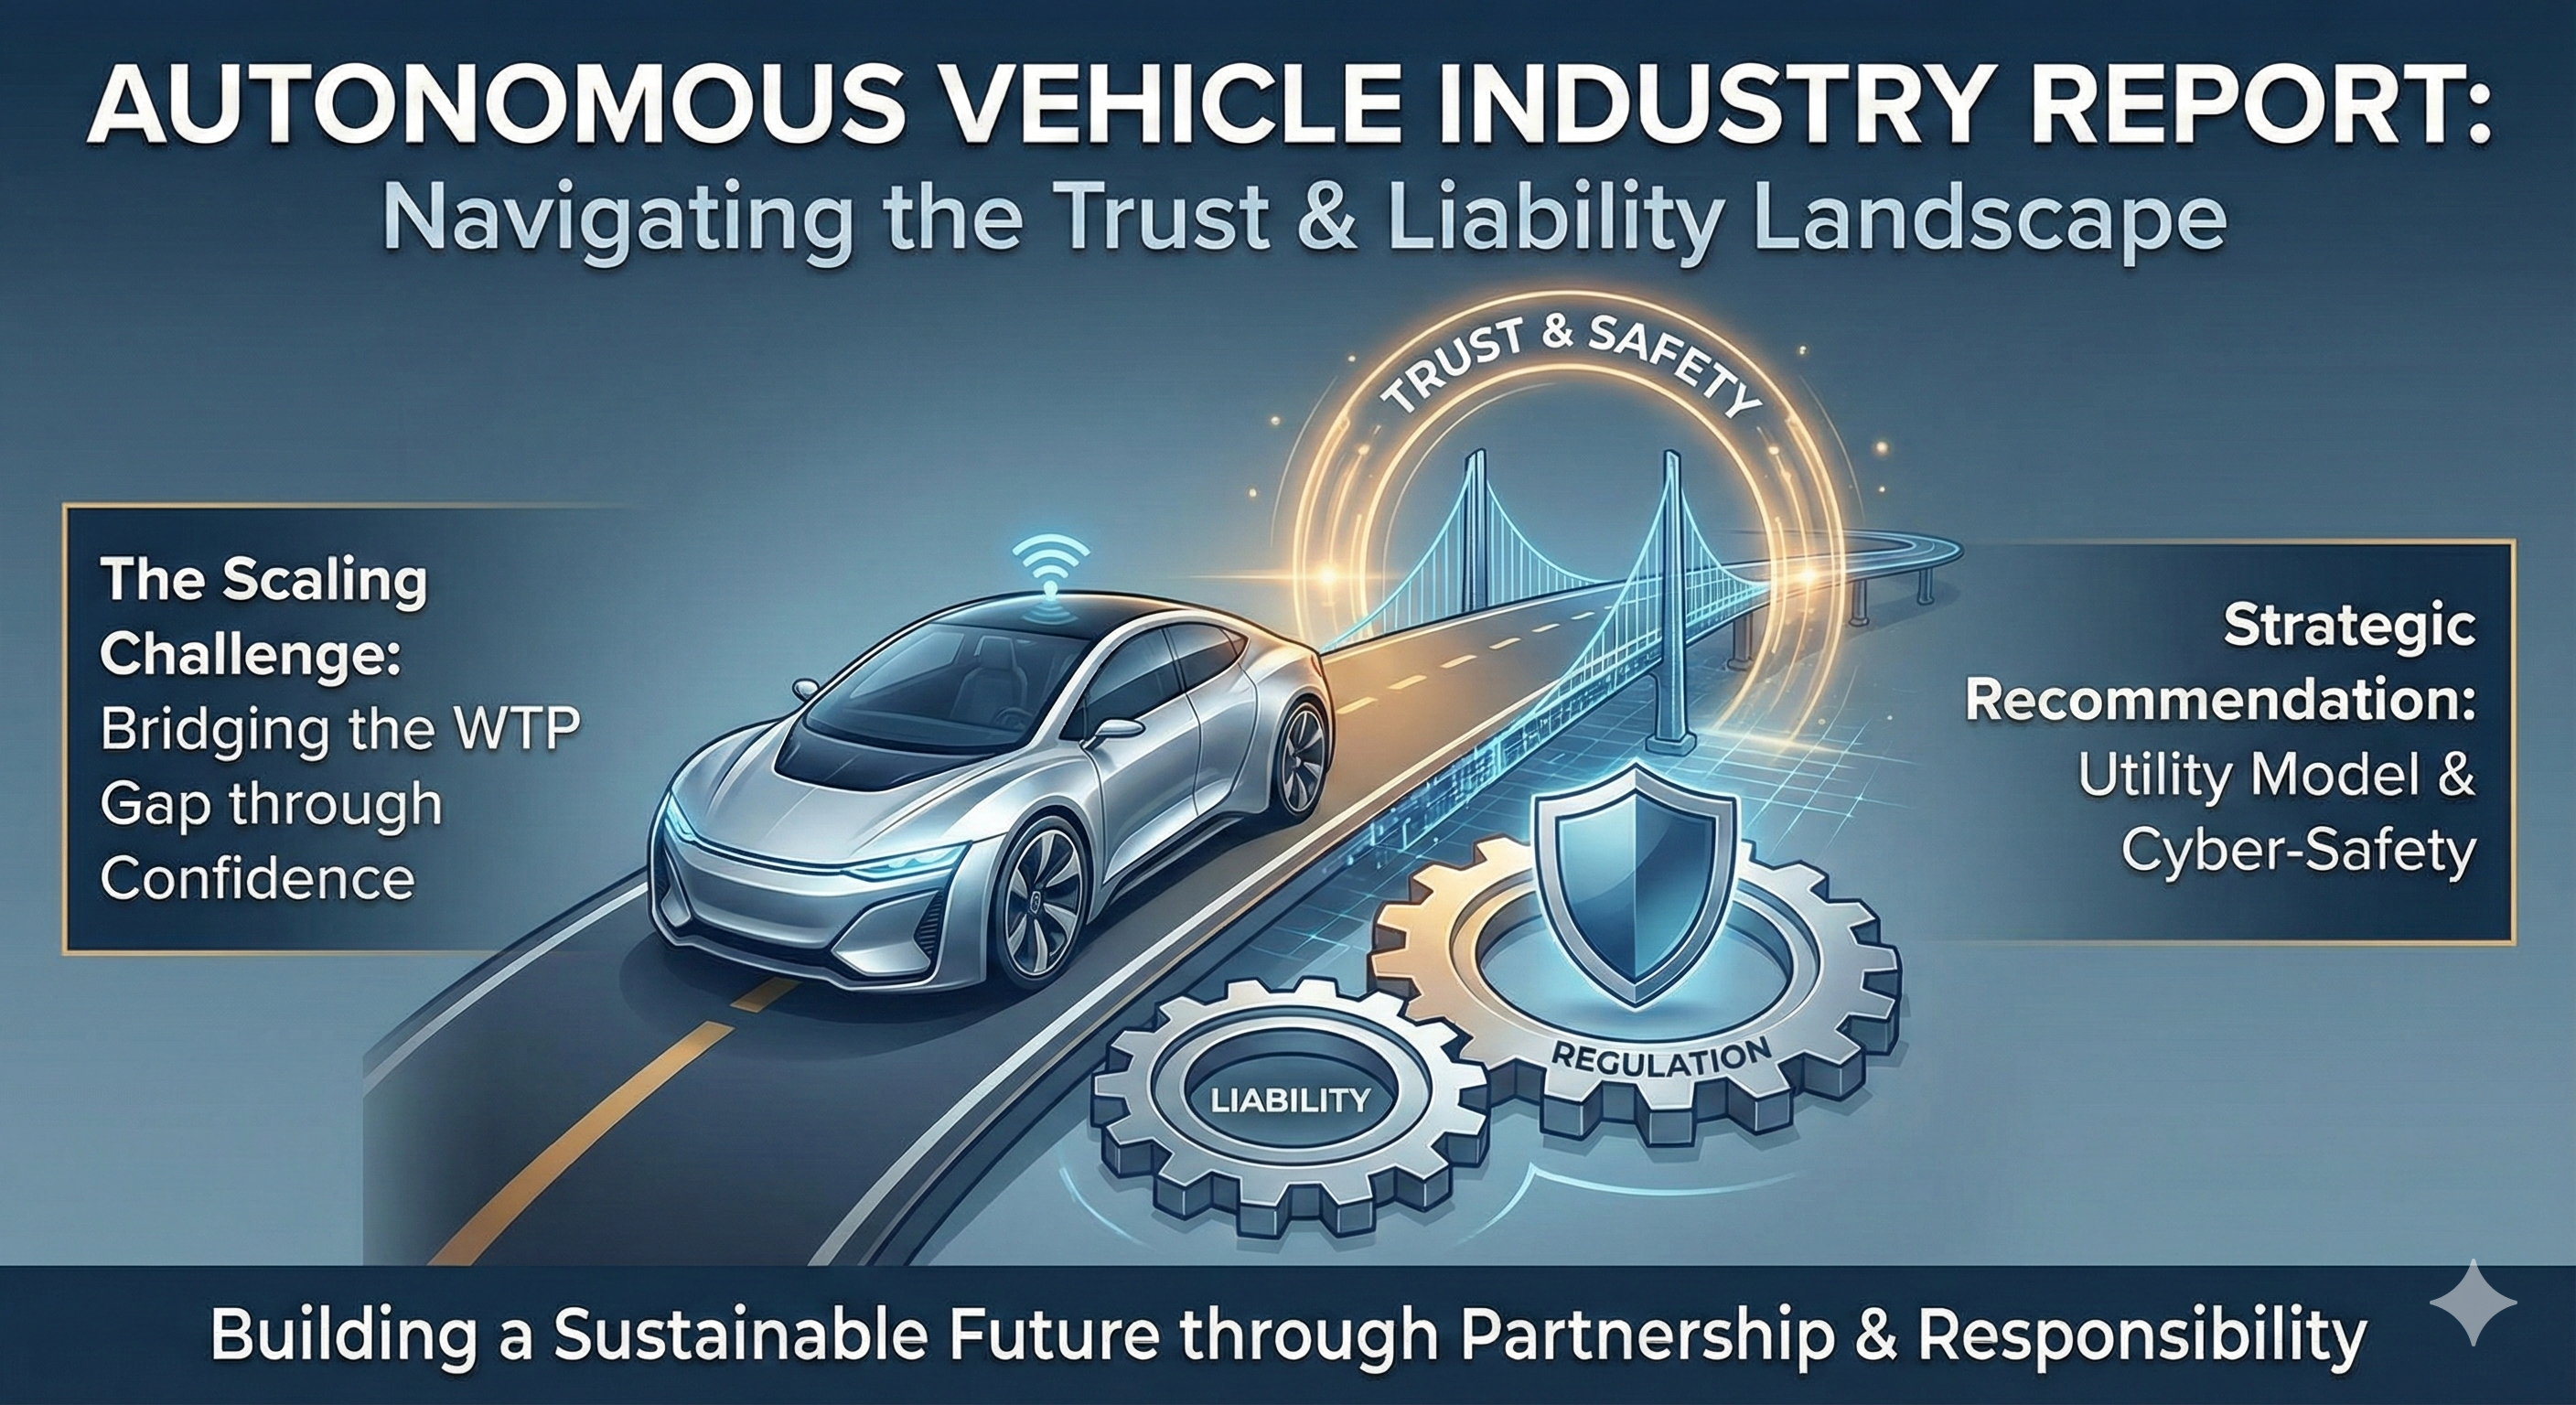
\includegraphics[width=1\linewidth,height=\textheight,keepaspectratio]{images/cover_image_av.png}
\end{center}

\bookmarksetup{startatroot}

\chapter*{Autonomous Vehicles: Strategy \&
Ethics}\label{autonomous-vehicles-strategy-ethics}
\addcontentsline{toc}{chapter}{Autonomous Vehicles: Strategy \& Ethics}

\markboth{Autonomous Vehicles: Strategy \& Ethics}{Autonomous Vehicles:
Strategy \& Ethics}

\textbf{A Data-Driven Analysis of the 2025 Consumer Landscape}

\section*{About This Report}\label{about-this-report}
\addcontentsline{toc}{section}{About This Report}

\markright{About This Report}

This interactive Quarto book serves as a comprehensive strategic review
of the Autonomous Vehicle (AV) industry. By combining macroeconomic
industry analysis with microeconomic consumer survey data, we aim to
answer two critical strategic questions:

\begin{enumerate}
\def\labelenumi{\arabic{enumi}.}
\tightlist
\item
  \textbf{How do we scale?} Determining the pricing power and adoption
  drivers for AV technology.
\item
  \textbf{What are the risks?} Understanding consumer fears, regulatory
  preferences, and ethical friction points.
\end{enumerate}

\section*{Objectives}\label{objectives}
\addcontentsline{toc}{section}{Objectives}

\markright{Objectives}

\begin{itemize}
\tightlist
\item
  \textbf{Industry Context:} Provide a high-level view of the market
  players, value proposition, and competitive forces.
\item
  \textbf{Objective 1 (Strategy):} Evaluate Willingness to Pay (WTP) and
  trust dynamics to formulate a scaling strategy.
\item
  \textbf{Objective 2 (Ethics):} Analyze public sentiment regarding
  regulation, accident liability, and safety risks.
\end{itemize}

\section*{Methodology}\label{methodology}
\addcontentsline{toc}{section}{Methodology}

\markright{Methodology}

This report utilizes R for statistical analysis, leveraging T-tests,
ANOVA, and Chi-Square tests to validate strategic insights derived from
a survey of \textasciitilde600 respondents.

\bookmarksetup{startatroot}

\chapter{Industry Strategic Review}\label{industry-strategic-review}

This section provides the macroeconomic context for the analysis,
evaluating the business landscape of the Autonomous Vehicle industry.

\section{Industry Overview}\label{industry-overview}

The Autonomous Vehicle (AV) industry is currently transitioning from the
``Trough of Disillusionment'' to the ``Slope of Enlightenment'' (Gartner
Hype Cycle). While early predictions of widespread Level 5 autonomy by
2020 failed to materialize, the market is now seeing tangible commercial
deployments in geofenced areas.

\begin{itemize}
\tightlist
\item
  \textbf{Market Size:} Estimated at \textasciitilde\$100 Billion in
  2024, projected to grow at a CAGR of \textgreater25\% through 2030.
\item
  \textbf{Key Shift:} The business model is shifting from \textbf{Asset
  Ownership} (selling cars to individuals) to
  \textbf{Transportation-as-a-Service (TaaS)} (selling rides via
  robotaxi fleets).
\end{itemize}

\begin{center}
\includegraphics[width=1\linewidth,height=\textheight,keepaspectratio]{images/Industry Strategic Review - visual selection.png}
\end{center}

\section{Major Players}\label{major-players}

The competitive landscape is bifurcated into two main approaches:

\begin{enumerate}
\def\labelenumi{\arabic{enumi}.}
\item
  \textbf{The ``Lidar \& Maps'' Camp (Robotaxis):}

  \begin{itemize}
  \tightlist
  \item
    \textbf{Waymo (Alphabet):} The current market leader with fully
    driverless commercial operations.
  \item
    \textbf{Cruise (GM):} A major player focusing on dense urban
    robotaxi fleets.
  \item
    \textbf{Zoox (Amazon):} Developing purpose-built carriages for urban
    transport.
  \end{itemize}
\item
  \textbf{The ``Vision-Only'' Camp (Consumer AV):}

  \begin{itemize}
  \tightlist
  \item
    \textbf{Tesla:} Pursuing a ``march of nines'' approach using
    camera-only data from consumer fleets to train neural networks.
  \end{itemize}
\end{enumerate}

\begin{center}
\includegraphics[width=1\linewidth,height=\textheight,keepaspectratio]{images/Industry Strategic Review - visual selection (1).png}
\end{center}

\section{Value Proposition}\label{value-proposition}

The value drivers differ by customer segment:

\begin{longtable}[]{@{}
  >{\raggedright\arraybackslash}p{(\linewidth - 2\tabcolsep) * \real{0.5000}}
  >{\raggedright\arraybackslash}p{(\linewidth - 2\tabcolsep) * \real{0.5000}}@{}}
\toprule\noalign{}
\begin{minipage}[b]{\linewidth}\raggedright
Segment
\end{minipage} & \begin{minipage}[b]{\linewidth}\raggedright
Primary Value Proposition
\end{minipage} \\
\midrule\noalign{}
\endhead
\bottomrule\noalign{}
\endlastfoot
\textbf{Consumer (Rider)} & \textbf{Safety:} Removing human error.
\textbf{Productivity:} Reclaiming commute time. \\
\textbf{Business (Operator)} & \textbf{Unit Economics:} Removing the
driver (approx. 70\% of ride cost). \textbf{Utilization:} 24/7 asset
uptime. \\
\end{longtable}

\begin{center}
\includegraphics[width=1\linewidth,height=\textheight,keepaspectratio]{images/Industry Strategic Review - visual selection (2).png}
\end{center}

\section{Porter's Five Forces
Analysis}\label{porters-five-forces-analysis}

\begin{enumerate}
\def\labelenumi{\arabic{enumi}.}
\tightlist
\item
  \textbf{Threat of New Entrants (Low):} Massive capital and data
  barriers.
\item
  \textbf{Bargaining Power of Suppliers (High):} Dependence on
  specialized chips (Nvidia) and sensors.
\item
  \textbf{Bargaining Power of Buyers (Medium):} Fleet operators have
  negotiating power; individual riders do not.
\item
  \textbf{Threat of Substitutes (High):} Remote work, public transit,
  and micromobility.
\item
  \textbf{Rivalry Among Competitors (High):} Winner-take-most dynamics
  for regulatory approval and network effects.
\end{enumerate}

\begin{center}
\includegraphics[width=1\linewidth,height=\textheight,keepaspectratio]{images/Industry Strategic Review - visual selection (3).png}
\end{center}

\section{Survey Data Overview}\label{survey-data-overview}

To validate these strategic assumptions, we use the
\texttt{AVsurvey.csv} dataset.

\begin{longtable}[]{@{}
  >{\raggedright\arraybackslash}p{(\linewidth - 134\tabcolsep) * \real{0.0152}}
  >{\raggedleft\arraybackslash}p{(\linewidth - 134\tabcolsep) * \real{0.0043}}
  >{\raggedleft\arraybackslash}p{(\linewidth - 134\tabcolsep) * \real{0.0061}}
  >{\raggedleft\arraybackslash}p{(\linewidth - 134\tabcolsep) * \real{0.0061}}
  >{\raggedleft\arraybackslash}p{(\linewidth - 134\tabcolsep) * \real{0.0061}}
  >{\raggedleft\arraybackslash}p{(\linewidth - 134\tabcolsep) * \real{0.0061}}
  >{\raggedleft\arraybackslash}p{(\linewidth - 134\tabcolsep) * \real{0.0061}}
  >{\raggedleft\arraybackslash}p{(\linewidth - 134\tabcolsep) * \real{0.0061}}
  >{\raggedright\arraybackslash}p{(\linewidth - 134\tabcolsep) * \real{0.0128}}
  >{\raggedright\arraybackslash}p{(\linewidth - 134\tabcolsep) * \real{0.0128}}
  >{\raggedright\arraybackslash}p{(\linewidth - 134\tabcolsep) * \real{0.0128}}
  >{\raggedright\arraybackslash}p{(\linewidth - 134\tabcolsep) * \real{0.0164}}
  >{\raggedright\arraybackslash}p{(\linewidth - 134\tabcolsep) * \real{0.0110}}
  >{\raggedright\arraybackslash}p{(\linewidth - 134\tabcolsep) * \real{0.0164}}
  >{\raggedright\arraybackslash}p{(\linewidth - 134\tabcolsep) * \real{0.0164}}
  >{\raggedright\arraybackslash}p{(\linewidth - 134\tabcolsep) * \real{0.0164}}
  >{\raggedright\arraybackslash}p{(\linewidth - 134\tabcolsep) * \real{0.0164}}
  >{\raggedleft\arraybackslash}p{(\linewidth - 134\tabcolsep) * \real{0.0128}}
  >{\raggedleft\arraybackslash}p{(\linewidth - 134\tabcolsep) * \real{0.0110}}
  >{\raggedleft\arraybackslash}p{(\linewidth - 134\tabcolsep) * \real{0.0091}}
  >{\raggedleft\arraybackslash}p{(\linewidth - 134\tabcolsep) * \real{0.0097}}
  >{\raggedright\arraybackslash}p{(\linewidth - 134\tabcolsep) * \real{0.0615}}
  >{\raggedleft\arraybackslash}p{(\linewidth - 134\tabcolsep) * \real{0.0103}}
  >{\raggedleft\arraybackslash}p{(\linewidth - 134\tabcolsep) * \real{0.0128}}
  >{\raggedleft\arraybackslash}p{(\linewidth - 134\tabcolsep) * \real{0.0097}}
  >{\raggedright\arraybackslash}p{(\linewidth - 134\tabcolsep) * \real{0.0128}}
  >{\raggedleft\arraybackslash}p{(\linewidth - 134\tabcolsep) * \real{0.0146}}
  >{\raggedleft\arraybackslash}p{(\linewidth - 134\tabcolsep) * \real{0.0146}}
  >{\raggedleft\arraybackslash}p{(\linewidth - 134\tabcolsep) * \real{0.0146}}
  >{\raggedleft\arraybackslash}p{(\linewidth - 134\tabcolsep) * \real{0.0146}}
  >{\raggedleft\arraybackslash}p{(\linewidth - 134\tabcolsep) * \real{0.0146}}
  >{\raggedleft\arraybackslash}p{(\linewidth - 134\tabcolsep) * \real{0.0146}}
  >{\raggedleft\arraybackslash}p{(\linewidth - 134\tabcolsep) * \real{0.0146}}
  >{\raggedright\arraybackslash}p{(\linewidth - 134\tabcolsep) * \real{0.0231}}
  >{\raggedright\arraybackslash}p{(\linewidth - 134\tabcolsep) * \real{0.0116}}
  >{\raggedright\arraybackslash}p{(\linewidth - 134\tabcolsep) * \real{0.0152}}
  >{\raggedright\arraybackslash}p{(\linewidth - 134\tabcolsep) * \real{0.0231}}
  >{\raggedright\arraybackslash}p{(\linewidth - 134\tabcolsep) * \real{0.0152}}
  >{\raggedright\arraybackslash}p{(\linewidth - 134\tabcolsep) * \real{0.0231}}
  >{\raggedright\arraybackslash}p{(\linewidth - 134\tabcolsep) * \real{0.0152}}
  >{\raggedright\arraybackslash}p{(\linewidth - 134\tabcolsep) * \real{0.0152}}
  >{\raggedright\arraybackslash}p{(\linewidth - 134\tabcolsep) * \real{0.0152}}
  >{\raggedright\arraybackslash}p{(\linewidth - 134\tabcolsep) * \real{0.0231}}
  >{\raggedright\arraybackslash}p{(\linewidth - 134\tabcolsep) * \real{0.0262}}
  >{\raggedright\arraybackslash}p{(\linewidth - 134\tabcolsep) * \real{0.0329}}
  >{\raggedright\arraybackslash}p{(\linewidth - 134\tabcolsep) * \real{0.0164}}
  >{\raggedright\arraybackslash}p{(\linewidth - 134\tabcolsep) * \real{0.0140}}
  >{\raggedright\arraybackslash}p{(\linewidth - 134\tabcolsep) * \real{0.0116}}
  >{\raggedright\arraybackslash}p{(\linewidth - 134\tabcolsep) * \real{0.0140}}
  >{\raggedright\arraybackslash}p{(\linewidth - 134\tabcolsep) * \real{0.0140}}
  >{\raggedright\arraybackslash}p{(\linewidth - 134\tabcolsep) * \real{0.0116}}
  >{\raggedright\arraybackslash}p{(\linewidth - 134\tabcolsep) * \real{0.0164}}
  >{\raggedright\arraybackslash}p{(\linewidth - 134\tabcolsep) * \real{0.0164}}
  >{\raggedright\arraybackslash}p{(\linewidth - 134\tabcolsep) * \real{0.0164}}
  >{\raggedright\arraybackslash}p{(\linewidth - 134\tabcolsep) * \real{0.0164}}
  >{\raggedright\arraybackslash}p{(\linewidth - 134\tabcolsep) * \real{0.0164}}
  >{\raggedright\arraybackslash}p{(\linewidth - 134\tabcolsep) * \real{0.0164}}
  >{\raggedright\arraybackslash}p{(\linewidth - 134\tabcolsep) * \real{0.0158}}
  >{\raggedright\arraybackslash}p{(\linewidth - 134\tabcolsep) * \real{0.0122}}
  >{\raggedright\arraybackslash}p{(\linewidth - 134\tabcolsep) * \real{0.0055}}
  >{\raggedright\arraybackslash}p{(\linewidth - 134\tabcolsep) * \real{0.0347}}
  >{\raggedright\arraybackslash}p{(\linewidth - 134\tabcolsep) * \real{0.0043}}
  >{\raggedright\arraybackslash}p{(\linewidth - 134\tabcolsep) * \real{0.0103}}
  >{\raggedright\arraybackslash}p{(\linewidth - 134\tabcolsep) * \real{0.0091}}
  >{\raggedright\arraybackslash}p{(\linewidth - 134\tabcolsep) * \real{0.0140}}
  >{\raggedright\arraybackslash}p{(\linewidth - 134\tabcolsep) * \real{0.0177}}
  >{\raggedright\arraybackslash}p{(\linewidth - 134\tabcolsep) * \real{0.0091}}
  >{\raggedright\arraybackslash}p{(\linewidth - 134\tabcolsep) * \real{0.0085}}@{}}
\caption{Survey Data Preview (Static Sample)}\tabularnewline
\toprule\noalign{}
\begin{minipage}[b]{\linewidth}\raggedright
participant\_id
\end{minipage} & \begin{minipage}[b]{\linewidth}\raggedleft
maxpay
\end{minipage} & \begin{minipage}[b]{\linewidth}\raggedleft
maxfare\_1
\end{minipage} & \begin{minipage}[b]{\linewidth}\raggedleft
maxfare\_2
\end{minipage} & \begin{minipage}[b]{\linewidth}\raggedleft
maxfare\_3
\end{minipage} & \begin{minipage}[b]{\linewidth}\raggedleft
maxfare\_4
\end{minipage} & \begin{minipage}[b]{\linewidth}\raggedleft
maxfare\_5
\end{minipage} & \begin{minipage}[b]{\linewidth}\raggedleft
maxfare\_7
\end{minipage} & \begin{minipage}[b]{\linewidth}\raggedright
conf\_right
\end{minipage} & \begin{minipage}[b]{\linewidth}\raggedright
conf\_safetech
\end{minipage} & \begin{minipage}[b]{\linewidth}\raggedright
conf\_safe
\end{minipage} & \begin{minipage}[b]{\linewidth}\raggedright
supportl\_dv\_1
\end{minipage} & \begin{minipage}[b]{\linewidth}\raggedright
supportl\_dv\_2
\end{minipage} & \begin{minipage}[b]{\linewidth}\raggedright
supportl\_dv\_3
\end{minipage} & \begin{minipage}[b]{\linewidth}\raggedright
supportl\_dv\_4
\end{minipage} & \begin{minipage}[b]{\linewidth}\raggedright
supportl\_dv\_5
\end{minipage} & \begin{minipage}[b]{\linewidth}\raggedright
supportl\_dv\_6
\end{minipage} & \begin{minipage}[b]{\linewidth}\raggedleft
acc\_blame\_programmer
\end{minipage} & \begin{minipage}[b]{\linewidth}\raggedleft
acc\_blame\_company
\end{minipage} & \begin{minipage}[b]{\linewidth}\raggedleft
acc\_blame\_govt
\end{minipage} & \begin{minipage}[b]{\linewidth}\raggedleft
acc\_blame\_other
\end{minipage} & \begin{minipage}[b]{\linewidth}\raggedright
acc\_blame\_other\_text
\end{minipage} & \begin{minipage}[b]{\linewidth}\raggedleft
reg\_focus\_safety
\end{minipage} & \begin{minipage}[b]{\linewidth}\raggedleft
reg\_focus\_innovation
\end{minipage} & \begin{minipage}[b]{\linewidth}\raggedleft
reg\_focus\_other
\end{minipage} & \begin{minipage}[b]{\linewidth}\raggedright
reg\_focus\_other\_text
\end{minipage} & \begin{minipage}[b]{\linewidth}\raggedleft
company\_purchase\_rank\_1
\end{minipage} & \begin{minipage}[b]{\linewidth}\raggedleft
company\_purchase\_rank\_2
\end{minipage} & \begin{minipage}[b]{\linewidth}\raggedleft
company\_purchase\_rank\_3
\end{minipage} & \begin{minipage}[b]{\linewidth}\raggedleft
company\_purchase\_rank\_4
\end{minipage} & \begin{minipage}[b]{\linewidth}\raggedleft
company\_purchase\_rank\_5
\end{minipage} & \begin{minipage}[b]{\linewidth}\raggedleft
company\_purchase\_rank\_6
\end{minipage} & \begin{minipage}[b]{\linewidth}\raggedleft
company\_purchase\_rank\_7
\end{minipage} & \begin{minipage}[b]{\linewidth}\raggedright
opinions
\end{minipage} & \begin{minipage}[b]{\linewidth}\raggedright
future
\end{minipage} & \begin{minipage}[b]{\linewidth}\raggedright
you\_alone
\end{minipage} & \begin{minipage}[b]{\linewidth}\raggedright
friends\_alone
\end{minipage} & \begin{minipage}[b]{\linewidth}\raggedright
family\_alone
\end{minipage} & \begin{minipage}[b]{\linewidth}\raggedright
stranger\_alone
\end{minipage} & \begin{minipage}[b]{\linewidth}\raggedright
you\_pass
\end{minipage} & \begin{minipage}[b]{\linewidth}\raggedright
friends\_pass
\end{minipage} & \begin{minipage}[b]{\linewidth}\raggedright
family\_pass
\end{minipage} & \begin{minipage}[b]{\linewidth}\raggedright
stranger\_pass
\end{minipage} & \begin{minipage}[b]{\linewidth}\raggedright
benefits\_oe
\end{minipage} & \begin{minipage}[b]{\linewidth}\raggedright
risks\_oe
\end{minipage} & \begin{minipage}[b]{\linewidth}\raggedright
media
\end{minipage} & \begin{minipage}[b]{\linewidth}\raggedright
drive
\end{minipage} & \begin{minipage}[b]{\linewidth}\raggedright
taxi
\end{minipage} & \begin{minipage}[b]{\linewidth}\raggedright
publictransit
\end{minipage} & \begin{minipage}[b]{\linewidth}\raggedright
bike
\end{minipage} & \begin{minipage}[b]{\linewidth}\raggedright
attn2
\end{minipage} & \begin{minipage}[b]{\linewidth}\raggedright
firstmover\_1
\end{minipage} & \begin{minipage}[b]{\linewidth}\raggedright
firstmover\_2
\end{minipage} & \begin{minipage}[b]{\linewidth}\raggedright
firstmover\_3
\end{minipage} & \begin{minipage}[b]{\linewidth}\raggedright
firstmover\_4
\end{minipage} & \begin{minipage}[b]{\linewidth}\raggedright
firstmover\_5
\end{minipage} & \begin{minipage}[b]{\linewidth}\raggedright
firstmover\_6r
\end{minipage} & \begin{minipage}[b]{\linewidth}\raggedright
race
\end{minipage} & \begin{minipage}[b]{\linewidth}\raggedright
edu
\end{minipage} & \begin{minipage}[b]{\linewidth}\raggedright
status
\end{minipage} & \begin{minipage}[b]{\linewidth}\raggedright
Employment.Status
\end{minipage} & \begin{minipage}[b]{\linewidth}\raggedright
Sex
\end{minipage} & \begin{minipage}[b]{\linewidth}\raggedright
Country.of.Birth
\end{minipage} & \begin{minipage}[b]{\linewidth}\raggedright
First.Language
\end{minipage} & \begin{minipage}[b]{\linewidth}\raggedright
Ethnicity..Simplified.
\end{minipage} & \begin{minipage}[b]{\linewidth}\raggedright
Current.Country.of.Residence
\end{minipage} & \begin{minipage}[b]{\linewidth}\raggedright
Student.Status
\end{minipage} & \begin{minipage}[b]{\linewidth}\raggedright
Nationality
\end{minipage} \\
\midrule\noalign{}
\endfirsthead
\toprule\noalign{}
\begin{minipage}[b]{\linewidth}\raggedright
participant\_id
\end{minipage} & \begin{minipage}[b]{\linewidth}\raggedleft
maxpay
\end{minipage} & \begin{minipage}[b]{\linewidth}\raggedleft
maxfare\_1
\end{minipage} & \begin{minipage}[b]{\linewidth}\raggedleft
maxfare\_2
\end{minipage} & \begin{minipage}[b]{\linewidth}\raggedleft
maxfare\_3
\end{minipage} & \begin{minipage}[b]{\linewidth}\raggedleft
maxfare\_4
\end{minipage} & \begin{minipage}[b]{\linewidth}\raggedleft
maxfare\_5
\end{minipage} & \begin{minipage}[b]{\linewidth}\raggedleft
maxfare\_7
\end{minipage} & \begin{minipage}[b]{\linewidth}\raggedright
conf\_right
\end{minipage} & \begin{minipage}[b]{\linewidth}\raggedright
conf\_safetech
\end{minipage} & \begin{minipage}[b]{\linewidth}\raggedright
conf\_safe
\end{minipage} & \begin{minipage}[b]{\linewidth}\raggedright
supportl\_dv\_1
\end{minipage} & \begin{minipage}[b]{\linewidth}\raggedright
supportl\_dv\_2
\end{minipage} & \begin{minipage}[b]{\linewidth}\raggedright
supportl\_dv\_3
\end{minipage} & \begin{minipage}[b]{\linewidth}\raggedright
supportl\_dv\_4
\end{minipage} & \begin{minipage}[b]{\linewidth}\raggedright
supportl\_dv\_5
\end{minipage} & \begin{minipage}[b]{\linewidth}\raggedright
supportl\_dv\_6
\end{minipage} & \begin{minipage}[b]{\linewidth}\raggedleft
acc\_blame\_programmer
\end{minipage} & \begin{minipage}[b]{\linewidth}\raggedleft
acc\_blame\_company
\end{minipage} & \begin{minipage}[b]{\linewidth}\raggedleft
acc\_blame\_govt
\end{minipage} & \begin{minipage}[b]{\linewidth}\raggedleft
acc\_blame\_other
\end{minipage} & \begin{minipage}[b]{\linewidth}\raggedright
acc\_blame\_other\_text
\end{minipage} & \begin{minipage}[b]{\linewidth}\raggedleft
reg\_focus\_safety
\end{minipage} & \begin{minipage}[b]{\linewidth}\raggedleft
reg\_focus\_innovation
\end{minipage} & \begin{minipage}[b]{\linewidth}\raggedleft
reg\_focus\_other
\end{minipage} & \begin{minipage}[b]{\linewidth}\raggedright
reg\_focus\_other\_text
\end{minipage} & \begin{minipage}[b]{\linewidth}\raggedleft
company\_purchase\_rank\_1
\end{minipage} & \begin{minipage}[b]{\linewidth}\raggedleft
company\_purchase\_rank\_2
\end{minipage} & \begin{minipage}[b]{\linewidth}\raggedleft
company\_purchase\_rank\_3
\end{minipage} & \begin{minipage}[b]{\linewidth}\raggedleft
company\_purchase\_rank\_4
\end{minipage} & \begin{minipage}[b]{\linewidth}\raggedleft
company\_purchase\_rank\_5
\end{minipage} & \begin{minipage}[b]{\linewidth}\raggedleft
company\_purchase\_rank\_6
\end{minipage} & \begin{minipage}[b]{\linewidth}\raggedleft
company\_purchase\_rank\_7
\end{minipage} & \begin{minipage}[b]{\linewidth}\raggedright
opinions
\end{minipage} & \begin{minipage}[b]{\linewidth}\raggedright
future
\end{minipage} & \begin{minipage}[b]{\linewidth}\raggedright
you\_alone
\end{minipage} & \begin{minipage}[b]{\linewidth}\raggedright
friends\_alone
\end{minipage} & \begin{minipage}[b]{\linewidth}\raggedright
family\_alone
\end{minipage} & \begin{minipage}[b]{\linewidth}\raggedright
stranger\_alone
\end{minipage} & \begin{minipage}[b]{\linewidth}\raggedright
you\_pass
\end{minipage} & \begin{minipage}[b]{\linewidth}\raggedright
friends\_pass
\end{minipage} & \begin{minipage}[b]{\linewidth}\raggedright
family\_pass
\end{minipage} & \begin{minipage}[b]{\linewidth}\raggedright
stranger\_pass
\end{minipage} & \begin{minipage}[b]{\linewidth}\raggedright
benefits\_oe
\end{minipage} & \begin{minipage}[b]{\linewidth}\raggedright
risks\_oe
\end{minipage} & \begin{minipage}[b]{\linewidth}\raggedright
media
\end{minipage} & \begin{minipage}[b]{\linewidth}\raggedright
drive
\end{minipage} & \begin{minipage}[b]{\linewidth}\raggedright
taxi
\end{minipage} & \begin{minipage}[b]{\linewidth}\raggedright
publictransit
\end{minipage} & \begin{minipage}[b]{\linewidth}\raggedright
bike
\end{minipage} & \begin{minipage}[b]{\linewidth}\raggedright
attn2
\end{minipage} & \begin{minipage}[b]{\linewidth}\raggedright
firstmover\_1
\end{minipage} & \begin{minipage}[b]{\linewidth}\raggedright
firstmover\_2
\end{minipage} & \begin{minipage}[b]{\linewidth}\raggedright
firstmover\_3
\end{minipage} & \begin{minipage}[b]{\linewidth}\raggedright
firstmover\_4
\end{minipage} & \begin{minipage}[b]{\linewidth}\raggedright
firstmover\_5
\end{minipage} & \begin{minipage}[b]{\linewidth}\raggedright
firstmover\_6r
\end{minipage} & \begin{minipage}[b]{\linewidth}\raggedright
race
\end{minipage} & \begin{minipage}[b]{\linewidth}\raggedright
edu
\end{minipage} & \begin{minipage}[b]{\linewidth}\raggedright
status
\end{minipage} & \begin{minipage}[b]{\linewidth}\raggedright
Employment.Status
\end{minipage} & \begin{minipage}[b]{\linewidth}\raggedright
Sex
\end{minipage} & \begin{minipage}[b]{\linewidth}\raggedright
Country.of.Birth
\end{minipage} & \begin{minipage}[b]{\linewidth}\raggedright
First.Language
\end{minipage} & \begin{minipage}[b]{\linewidth}\raggedright
Ethnicity..Simplified.
\end{minipage} & \begin{minipage}[b]{\linewidth}\raggedright
Current.Country.of.Residence
\end{minipage} & \begin{minipage}[b]{\linewidth}\raggedright
Student.Status
\end{minipage} & \begin{minipage}[b]{\linewidth}\raggedright
Nationality
\end{minipage} \\
\midrule\noalign{}
\endhead
\bottomrule\noalign{}
\endlastfoot
54f8b0cdfdf99b5396a7d0a2 & 12000 & 10 & 5 & 6 & 20 & 10 & 10 & Somewhat
confident & Not very confident & Somewhat confident & Neither agree nor
disagree & Somewhat agree & Somewhat disagree & Somewhat agree & Neither
agree nor disagree & Somewhat disagree & 32 & 36 & 32 & 0 & & 95 & 5 & 0
& & 3 & 2 & 1 & 4 & 7 & 5 & 6 & The general public & Within 5-10 years &
Moderately uncomfortable & Neither comfortable nor uncomfortable &
Slightly uncomfortable & Neither comfortable nor uncomfortable &
Moderately uncomfortable & Slightly uncomfortable & Slightly
uncomfortable & Neither comfortable nor uncomfortable & convenience,
traffic control, cost control & loss of privacy, loss of control,
hackers with malice & Within the past week & A few times per week & A
few times a year & A few times a year & A few times per week & A few
times a year & Somewhat agree & Somewhat agree & Somewhat agree &
Neither agree nor disagree & Neither agree nor disagree & Neither agree
nor disagree & White,Hispanic or Latinx & 4 year degree & 4th Rung &
Full-Time & Female & Uruguay & English & White & United States & No &
United States \\
55884984fdf99b4021921e67 & 15000 & 8 & 12 & 5 & 20 & 10 & 5 & Not
confident at all & Not very confident & Not very confident & Strongly
disagree & Disagree & Disagree & Neither agree nor disagree & Strongly
disagree & Strongly disagree & 71 & 28 & 1 & 0 & & 91 & 9 & 0 & & 3 & 1
& 4 & 2 & 7 & 5 & 6 & Experts in technology & Within 10-20 years &
Extremely uncomfortable & Extremely uncomfortable & Extremely
uncomfortable & Moderately uncomfortable & Moderately uncomfortable &
Moderately uncomfortable & Moderately uncomfortable & Slightly
uncomfortable & Able to relax & Getting in accidents & Within the past
year & A few times per week & A few times a year & Less than once a year
& A few times a year & A few times a year & Agree & Somewhat agree &
Somewhat agree & Neither agree nor disagree & Neither agree nor disagree
& Somewhat disagree & White & 2 year degree & 8th Rung & Part-Time &
Female & United States & English & White & United States & No & United
States \\
5589cf61fdf99b18bd86d076 & 0 & 20 & 0 & 20 & 20 & 0 & 0 & Not confident
at all & Not confident at all & Not confident at all & Strongly disagree
& Strongly disagree & Strongly disagree & Somewhat agree & Strongly
disagree & Somewhat disagree & 80 & 10 & 10 & 0 & & 95 & 5 & 0 & & 4 & 7
& 1 & 2 & 3 & 5 & 6 & The government & Within 5-10 years & Extremely
uncomfortable & Moderately uncomfortable & Extremely uncomfortable &
Slightly uncomfortable & Extremely uncomfortable & Moderately
uncomfortable & Extremely uncomfortable & Slightly uncomfortable &
increased fuel economy & risk of accidents & Within the past few months
& Daily & Never & Never & A few times per week & A few times a year &
Somewhat disagree & Somewhat disagree & Neither agree nor disagree &
Agree & Agree & Agree & White & 2 year degree & 7th Rung & Full-Time &
Female & United States & English & White & United States & No & United
States \\
559d9916fdf99b1e2b2dc6b8 & 0 & 0 & 0 & 0 & 20 & 0 & 0 & Not confident at
all & Not confident at all & Not confident at all & Strongly disagree &
Strongly disagree & Strongly disagree & Somewhat agree & Strongly
disagree & Strongly disagree & 50 & 0 & 0 & 50 & whatever other parties
were involved, for example drivers of other vehicles involved in the
accident & 100 & 0 & 0 & & 1 & 4 & 3 & 2 & 5 & 6 & 7 & Experts in ethics
and social problems & Within 20-50 years & Extremely uncomfortable &
Extremely uncomfortable & Extremely uncomfortable & Extremely
uncomfortable & Extremely uncomfortable & Extremely uncomfortable &
Extremely uncomfortable & Extremely uncomfortable & There are none. &
They are dangerous. & Within the past month & A few times per week &
Never & A few times each month & Daily & A few times a year & Strongly
disagree & Neither agree nor disagree & Neither agree nor disagree &
Agree & Strongly agree & Strongly agree & White & 4 year degree & 9th
Rung & Not in paid work (e.g.~homemaker', 'retired or disabled) & Female
& United States & English & White & United States & No & United
States \\
559ef308fdf99b2616ff2a4f & 8000 & 10 & 10 & 7 & 20 & 5 & 2 & Not very
confident & Somewhat confident & Somewhat confident & Somewhat agree &
Agree & Somewhat agree & Neither agree nor disagree & Neither agree nor
disagree & Neither agree nor disagree & 10 & 71 & 19 & 0 & & 100 & 0 & 0
& & 1 & 3 & 2 & 4 & 5 & 7 & 6 & The government & Within 5-10 years &
Slightly comfortable & Slightly comfortable & Slightly comfortable &
Slightly comfortable & Slightly comfortable & Slightly comfortable &
Slightly comfortable & Slightly comfortable & less driver error &
hacking by nefarious people & Within the past month & A few times per
week & A few times a year & A few times a year & A few times each month
& A few times a year & Neither agree nor disagree & Somewhat disagree &
Somewhat agree & Neither agree nor disagree & Somewhat agree & Somewhat
agree & White & Doctorate & 5th Rung & Part-Time & Female & United
States & English & White & United States & No & United States \\
55abb1a5fdf99b501fab62e3 & 20000 & 15 & 5 & 10 & 20 & 10 & 5 & Somewhat
confident & Somewhat confident & Somewhat confident & Somewhat agree &
Somewhat agree & Somewhat agree & Somewhat agree & Somewhat agree &
Neither agree nor disagree & 50 & 50 & 0 & 0 & & 80 & 20 & 0 & & 2 & 3 &
1 & 5 & 4 & 7 & 6 & Experts in technology & Within 10-20 years &
Slightly uncomfortable & Slightly uncomfortable & Slightly uncomfortable
& Slightly uncomfortable & Slightly uncomfortable & Slightly
uncomfortable & Slightly uncomfortable & Slightly uncomfortable &
safety, time, convenience & uncontrollable, anonymous, uncaring & Within
the past week & A few times per week & Never & Never & Daily & A few
times a year & Disagree & Disagree & Neither agree nor disagree & Agree
& Agree & Somewhat agree & White & Professional degree & 5th Rung &
Full-Time & Male & United States & English & White & United States & No
& United States \\
55b9a9b0fdf99b6906d2aba4 & 30000 & 10 & 10 & 5 & 20 & 5 & 1 & Very
confident & Very confident & Very confident & Strongly agree & Strongly
agree & Agree & Agree & Agree & Somewhat disagree & 5 & 90 & 5 & 0 & &
95 & 5 & 0 & & 1 & 2 & 3 & 7 & 6 & 4 & 5 & The government & Within 5-10
years & Moderately comfortable & Moderately comfortable & Moderately
comfortable & Moderately comfortable & Moderately comfortable &
Moderately comfortable & Moderately comfortable & Moderately comfortable
& independence, economy, convenience & safety, privacy, hacking & Within
the past month & A few times each month & Never & A few times a year & A
few times each month & A few times a year & Somewhat agree & Strongly
agree & Strongly agree & Agree & Strongly agree & Disagree & White &
Some college & 6th Rung & Not in paid work (e.g.~homemaker', 'retired or
disabled) & Male & United States & English & White & United States & No
& United States \\
561d98e03d7fe8000b0f5e09 & 30000 & 17 & 11 & 6 & 20 & 3 & 5 & Not very
confident & Not very confident & Not very confident & Somewhat agree &
Somewhat agree & Neither agree nor disagree & Strongly agree & Somewhat
disagree & Agree & 27 & 26 & 5 & 42 & & 88 & 12 & 0 & & 2 & 7 & 1 & 4 &
3 & 6 & 5 & Experts in technology & Within 5-10 years & Moderately
uncomfortable & Moderately uncomfortable & Moderately uncomfortable &
Moderately uncomfortable & Moderately uncomfortable & Moderately
uncomfortable & Moderately uncomfortable & Moderately uncomfortable &
convenient, futuristic, good & overconfidence, programming,people &
Within the past few months & A few times per week & Never & A few times
a year & Never & A few times a year & Somewhat disagree & Somewhat
disagree & Somewhat disagree & Somewhat agree & Somewhat agree &
Somewhat agree & White & Professional degree & 3rd Rung & Other & Female
& United States & English & White & United States & No & United
States \\
567dd32b4f0ef30006dbb718 & 0 & 8 & 0 & 8 & 20 & 8 & 3 & Somewhat
confident & Somewhat confident & Somewhat confident & Somewhat agree &
Agree & Agree & Disagree & Neither agree nor disagree & Neither agree
nor disagree & 70 & 30 & 0 & 0 & & 90 & 10 & 0 & & 1 & 7 & 2 & 4 & 3 & 5
& 6 & The government & Within 10-20 years & Slightly uncomfortable &
Slightly uncomfortable & Slightly uncomfortable & Slightly uncomfortable
& Slightly comfortable & Slightly comfortable & Slightly comfortable &
Slightly comfortable & More driver uniformity on the roads & Lack of
knowing how the vehicle may react & Within the past few months & Daily &
Never & Never & Daily & A few times a year & Somewhat disagree &
Somewhat disagree & Agree & Somewhat agree & Somewhat agree & Somewhat
agree & Black or African American & Professional degree & 7th Rung &
Full-Time & Female & United States & English & Black & United States &
No & United States \\
5687d85e369319000c269c55 & 50000 & 14 & 20 & 12 & 20 & 10 & 2 & Very
confident & Very confident & Very confident & Strongly agree & Strongly
agree & Strongly agree & Neither agree nor disagree & Neither agree nor
disagree & Neither agree nor disagree & 41 & 40 & 19 & 0 & & 60 & 40 & 0
& & 2 & 7 & 1 & 4 & 5 & 6 & 3 & The general public & Within 10-20 years
& Extremely comfortable & Extremely comfortable & Extremely comfortable
& Extremely comfortable & Extremely comfortable & Extremely comfortable
& Extremely comfortable & Extremely comfortable & Reduction of accidents
& Lack of control & Within the past month & Daily & Once a month & Once
a month & Once a month & A few times a year & Strongly agree & Strongly
agree & Agree & Neither agree nor disagree & Strongly agree & Agree &
Asian & 4 year degree & 8th Rung & Full-Time & Male & United States &
Chinese & Asian & United States & No & United States \\
\end{longtable}

\bookmarksetup{startatroot}

\chapter{Objective 1: Strategy for
Scaling}\label{objective-1-strategy-for-scaling}

\textbf{Goal:} Determine a strategy for scaling autonomous vehicles by
analyzing consumer Willingness to Pay (WTP) and confidence drivers.

\section{The Pricing Gap: Human
vs.~AV}\label{the-pricing-gap-human-vs.-av}

\textbf{Question}: Does the market demand a discount for AVs, or will
they pay a premium?

\begin{figure}

\centering{

\pandocbounded{\includegraphics[keepaspectratio]{objectives_1_files/figure-pdf/fig-wtp-comp-1.pdf}}

}

\caption{\label{fig-wtp-comp}WTP Comparison: Private Human
vs.~Autonomous Vehicles}

\end{figure}%

\begin{table}
\caption*{
{\fontsize{20}{25}\selectfont  Paired T-Test: Private Human vs. AV\fontsize{12}{15}\selectfont }
} 
\fontsize{12.0pt}{14.0pt}\selectfont
\begin{tabular*}{\linewidth}{@{\extracolsep{\fill}}rrrrr}
\toprule
Mean Diff & t-statistic & P-Value & 95\% CI Lower & 95\% CI Upper \\ 
\midrule\addlinespace[2.5pt]
2.74 & 8.91 & 0.000 & 2.14 & 3.34 \\ 
\bottomrule
\end{tabular*}
\end{table}

\textbf{Analysis}: If the mean WTP for AVs is lower, the strategy must
initially focus on cost-leadership or subsidization to drive adoption.
Here, we see a significant difference in WTP, indicating consumers
expect a discount for AV rides.

\section{Tech Savviness and WTP}\label{tech-savviness-and-wtp}

\textbf{Question:} \emph{How do consumers' WTP for rides driven
autonomously vary by their own tech savviness?}

\begin{figure}

\centering{

\pandocbounded{\includegraphics[keepaspectratio]{objectives_1_files/figure-pdf/fig-tech-savvy-1.pdf}}

}

\caption{\label{fig-tech-savvy}WTP by Tech Savviness Level}

\end{figure}%

\begin{table}
\fontsize{12.0pt}{14.0pt}\selectfont
\begin{tabular*}{\linewidth}{@{\extracolsep{\fill}}lccccccc}
\toprule
\textbf{Tech Confidence} & \textbf{N} & \textbf{Completely confident}  N = 13 & \textbf{Not confident at all}  N = 40 & \textbf{Not very confident}  N = 103 & \textbf{Somewhat confident}  N = 196 & \textbf{Very confident}  N = 91 & \textbf{p-value}\textsuperscript{\textit{1}} \\ 
\midrule\addlinespace[2.5pt]
{\bfseries WTP (\$), Mean (SD)} & 443 & 11.38 (5.85) & 2.10 (4.69) & 6.67 (7.03) & 9.29 (6.85) & 11.40 (7.21) & <0.001 \\ 
\bottomrule
\end{tabular*}
\begin{minipage}{\linewidth}
\textsuperscript{\textit{1}}One-way analysis of means\\
\end{minipage}
\end{table}

\emph{Analysis:} A significant ANOVA here indicates that tech-savvy
consumers are more willing to pay for AV rides. This suggests targeted
marketing and early adoption strategies should focus on this demographic
to build initial traction.

\section{Demographic Analysis:
Gender}\label{demographic-analysis-gender}

\textbf{Question:} \emph{How does WTP vary by Gender?}

\begin{figure}

\centering{

\pandocbounded{\includegraphics[keepaspectratio]{objectives_1_files/figure-pdf/fig-gender-wtp-1.pdf}}

}

\caption{\label{fig-gender-wtp}WTP for Private AV by Gender}

\end{figure}%

\begin{table}
\fontsize{12.0pt}{14.0pt}\selectfont
\begin{tabular*}{\linewidth}{@{\extracolsep{\fill}}lccc}
\toprule
\textbf{Characteristic} & \textbf{Female}  N = 240 & \textbf{Male}  N = 202 & \textbf{p-value}\textsuperscript{\textit{1}} \\ 
\midrule\addlinespace[2.5pt]
{\bfseries WTP (\$), Mean (SD)} & 8 (7) & 9 (7) & 0.17 \\ 
\bottomrule
\end{tabular*}
\begin{minipage}{\linewidth}
\textsuperscript{\textit{1}}Wilcoxon rank sum test\\
\end{minipage}
\end{table}

\textbf{Analysis:} There is no significant difference in WTP by gender,
indicating that pricing strategies do not need to be gender-specific.
This suggests a uniform pricing approach across genders is appropriate.

\section{Private vs.~Shared Dynamics}\label{private-vs.-shared-dynamics}

\textbf{Question:} \emph{How does the WTP degradation compare when
moving from Private to Shared?}

\begin{figure}

\centering{

\pandocbounded{\includegraphics[keepaspectratio]{objectives_1_files/figure-pdf/fig-wtp-shared-1.pdf}}

}

\caption{\label{fig-wtp-shared}WTP Comparison: Shared Human vs.~Shared
Autonomous Vehicles}

\end{figure}%

\begin{table}
\caption*{
{\fontsize{20}{25}\selectfont  Paired T-Test: Shared Human vs. AV\fontsize{12}{15}\selectfont }
} 
\fontsize{12.0pt}{14.0pt}\selectfont
\begin{tabular*}{\linewidth}{@{\extracolsep{\fill}}rrrrr}
\toprule
Mean Diff & t-statistic & P-Value & 95\% CI Lower & 95\% CI Upper \\ 
\midrule\addlinespace[2.5pt]
-12.28 & -44.77 & 0.000 & -12.82 & -11.74 \\ 
\bottomrule
\end{tabular*}
\end{table}

\emph{Analysis:} Comparing the WTP drop from Private to Shared for both
Human and AV modes reveals insights into consumer preferences for
ride-sharing in the context of autonomous technology. Here we see if the
shared model further depresses WTP significantly.

\section{The Trust Premium (Safety)}\label{the-trust-premium-safety}

\textbf{Question:} \emph{Can we charge more if consumers trust the
safety technology?}

\begin{figure}

\centering{

\pandocbounded{\includegraphics[keepaspectratio]{objectives_1_files/figure-pdf/fig-conf-safe-1.pdf}}

}

\caption{\label{fig-conf-safe}WTP by Safety Confidence Level}

\end{figure}%

\begin{table}
\fontsize{12.0pt}{14.0pt}\selectfont
\begin{tabular*}{\linewidth}{@{\extracolsep{\fill}}lccccccc}
\toprule
\textbf{Variable} & \textbf{N} & \textbf{Completely confident}  N = 8 & \textbf{Not confident at all}  N = 46 & \textbf{Not very confident}  N = 115 & \textbf{Somewhat confident}  N = 192 & \textbf{Very confident}  N = 82 & \textbf{p-value}\textsuperscript{\textit{1}} \\ 
\midrule\addlinespace[2.5pt]
{\bfseries WTP for Private AV (\$), Mean (SD)} & 443 & 12.25 (9.81) & 3.22 (6.36) & 6.51 (6.73) & 9.43 (6.53) & 11.84 (7.36) & <0.001 \\ 
\bottomrule
\end{tabular*}
\begin{minipage}{\linewidth}
\textsuperscript{\textit{1}}One-way analysis of means\\
\end{minipage}
\end{table}

\emph{Analysis:} A significant ANOVA suggests that marketing spend on
safety demonstration is directly convertible to higher fares. Here we
assess if higher confidence in safety correlates with increased WTP for
AV rides. In general, higher confidence should lead to higher WTP. Thus,
safety trust-building is a key scaling lever.

\section{The Ethics Premium}\label{the-ethics-premium}

\textbf{Question:} \emph{Does trust in ethical algorithms drive value as
much as physical safety?}

\begin{figure}

\centering{

\pandocbounded{\includegraphics[keepaspectratio]{objectives_1_files/figure-pdf/fig-conf-ethics-1.pdf}}

}

\caption{\label{fig-conf-ethics}WTP by Ethical Confidence Level}

\end{figure}%

\begin{table}
\fontsize{12.0pt}{14.0pt}\selectfont
\begin{tabular*}{\linewidth}{@{\extracolsep{\fill}}lccccccc}
\toprule
\textbf{Variable} & \textbf{N} & \textbf{Completely confident}  N = 9 & \textbf{Not confident at all}  N = 93 & \textbf{Not very confident}  N = 165 & \textbf{Somewhat confident}  N = 126 & \textbf{Very confident}  N = 50 & \textbf{p-value}\textsuperscript{\textit{1}} \\ 
\midrule\addlinespace[2.5pt]
{\bfseries WTP for Private AV (\$), Mean (SD)} & 443 & 13.67 (9.55) & 5.09 (6.87) & 7.65 (5.81) & 10.56 (7.60) & 11.76 (7.50) & <0.001 \\ 
\bottomrule
\end{tabular*}
\begin{minipage}{\linewidth}
\textsuperscript{\textit{1}}One-way analysis of means\\
\end{minipage}
\end{table}

\emph{Analysis:} If the ANOVA for ethical confidence is significant but
with a lower F-value than safety, it indicates that while ethics matter,
safety is the primary trust driver for WTP. Thus, ethical assurances are
secondary to physical safety in scaling strategy, but here we quantify
that impact and see that ethics still plays a role.

\section{Confidence \& WTP: Safety
vs.~Ethics}\label{confidence-wtp-safety-vs.-ethics}

\textbf{Question:} \emph{How do consumers' WTP change with their
confidence in the capacity of AV to keep them safe? And how does it
change with their confidence in AV to make the right choice in ethical
dilemmas?}

\begin{figure}

\centering{

\pandocbounded{\includegraphics[keepaspectratio]{objectives_1_files/figure-pdf/fig-safety-ethics-comparison-1.pdf}}

}

\caption{\label{fig-safety-ethics-comparison}WTP by Saftey and Ethics}

\end{figure}%

\begin{table}
\fontsize{12.0pt}{14.0pt}\selectfont
\begin{tabular*}{\linewidth}{@{\extracolsep{\fill}}lcccccccccccc}
\toprule
 & \multicolumn{6}{c}{\textbf{Safety Confidence}} & \multicolumn{6}{c}{\textbf{Ethical Confidence}} \\ 
\cmidrule(lr){2-7} \cmidrule(lr){8-13}
\textbf{Characteristic} & \textbf{Completely confident}  N = 8 & \textbf{Not confident at all}  N = 46 & \textbf{Not very confident}  N = 115 & \textbf{Somewhat confident}  N = 192 & \textbf{Very confident}  N = 82 & \textbf{p-value}\textsuperscript{\textit{1}} & \textbf{Completely confident}  N = 9 & \textbf{Not confident at all}  N = 93 & \textbf{Not very confident}  N = 165 & \textbf{Somewhat confident}  N = 126 & \textbf{Very confident}  N = 50 & \textbf{p-value}\textsuperscript{\textit{1}} \\ 
\midrule\addlinespace[2.5pt]
WTP (Safety Sort), Median (IQR) & 10 (5 \textendash 18) & 0 (0 \textendash 3) & 5 (0 \textendash 10) & 9 (5 \textendash 12) & 10 (6 \textendash 15) & <0.001 &  &  &  &  &  &  \\ 
WTP (Ethics Sort) &  &  &  &  &  &  & 10 (6 \textendash 22) & 1 (0 \textendash 8) & 7 (4 \textendash 10) & 9 (5 \textendash 14) & 10 (5 \textendash 17) & <0.001 \\ 
\bottomrule
\end{tabular*}
\begin{minipage}{\linewidth}
\textsuperscript{\textit{1}}Kruskal-Wallis rank sum test\\
\end{minipage}
\end{table}

\textbf{Analysis:} This side-by-side comparison highlights which
dimension of trust (safety vs.~ethics) has a stronger influence on WTP.
The results can guide prioritization in trust-building efforts. It
appears both have significant effects, but safety likely has a stronger
impact.

\section{Company Preference Leaders}\label{company-preference-leaders}

\textbf{Question:} \emph{Which companies do consumers prefer to be the
leaders in the AV industry?}

We analyze the ranking data where consumers ranked 7 companies from 1
(Most Preferred) to 7 (Least Preferred). Lower values indicate higher
preference.

\pandocbounded{\includegraphics[keepaspectratio]{objectives_1_files/figure-pdf/tab-trust-comparison-1.pdf}}

\textbf{Analysis:} The ranking data provides insights into which
companies are perceived as leaders in AV technology. Companies that rank
higher may have a competitive advantage in consumer trust, which can be
leveraged in marketing and partnership strategies. Here based on Average
preference rank, we can identify which companies are leading in consumer
trust and preference. Here company 1 appears to be the leader.

\section{Impact of Tech Savviness on Company
Preference}\label{impact-of-tech-savviness-on-company-preference}

\textbf{Question:} \emph{How do consumers' preferences change if they
are very tech savvy vs.~not very tech savvy?}

\begin{figure}

\centering{

\pandocbounded{\includegraphics[keepaspectratio]{objectives_1_files/figure-pdf/fig-company-rank-tech-1.pdf}}

}

\caption{\label{fig-company-rank-tech}Company Preference by Tech
Savviness}

\end{figure}%

\begin{table}
\fontsize{12.0pt}{14.0pt}\selectfont
\begin{tabular*}{\linewidth}{@{\extracolsep{\fill}}lcccccc}
\toprule
\textbf{Preferred Company} & \textbf{Completely confident}  N = 13 & \textbf{Not confident at all}  N = 37 & \textbf{Not very confident}  N = 99 & \textbf{Somewhat confident}  N = 187 & \textbf{Very confident}  N = 89 & \textbf{p-value}\textsuperscript{\textit{1}} \\ 
\midrule\addlinespace[2.5pt]
{\bfseries Preferred Company (Rank 1), n (\%)} &  &  &  &  &  & 0.002 \\ 
    Company 1 & 10 (77) & 9 (24) & 36 (36) & 99 (53) & 58 (65) &  \\ 
    Company 2 & 1 (7.7) & 6 (16) & 16 (16) & 15 (8.0) & 2 (2.2) &  \\ 
    Company 3 & 0 (0) & 16 (43) & 35 (35) & 49 (26) & 17 (19) &  \\ 
    Company 4 & 2 (15) & 2 (5.4) & 8 (8.1) & 11 (5.9) & 6 (6.7) &  \\ 
    Company 5 & 0 (0) & 4 (11) & 3 (3.0) & 12 (6.4) & 4 (4.5) &  \\ 
    Company 6 & 0 (0) & 0 (0) & 0 (0) & 0 (0) & 1 (1.1) &  \\ 
    Company 7 & 0 (0) & 0 (0) & 1 (1.0) & 1 (0.5) & 1 (1.1) &  \\ 
\bottomrule
\end{tabular*}
\begin{minipage}{\linewidth}
\textsuperscript{\textit{1}}Pearson's Chi-squared test\\
\end{minipage}
\end{table}

\section{Strategic Synthesis for
Scaling}\label{strategic-synthesis-for-scaling}

Based on the data above:

\begin{enumerate}
\def\labelenumi{\arabic{enumi}.}
\item
  \textbf{Pricing:} As WTP is lower for AVs, AV firms should enter the
  market with competitive pricing. If the WTP gap is large, they should
  consider subsidies or promotions to drive initial adoption and build a
  safety record. This will help overcome the initial trust barrier and
  have consumers experience the technology firsthand.
\item
  \textbf{Marketing:} Prioritize ``Safety'' messaging over ``Ethics'' as
  the ANOVA F-value for safety is higher. Thus, investments in safety
  demonstrations, transparent safety records, and endorsements from
  safety authorities will yield higher returns in consumer trust and
  WTP. If resources allow, ethical assurances can be secondary
  messaging.
\item
  \textbf{Product Mix:} As the gap between Private AV and Shared AV is
  small, push Shared AVs to maximize fleet revenue per mile.
\item
  \textbf{Trust-Building:} Implement programs to increase consumer
  confidence in AV safety, such as offering test rides, transparent
  reporting of safety metrics, and third-party safety certifications.
  This will directly translate into higher WTP and faster scaling.
\item
  \textbf{Continuous Monitoring:} Regularly survey consumer confidence
  and WTP to adapt pricing and marketing strategies as the market
  matures and trust builds over time.
\end{enumerate}

\bookmarksetup{startatroot}

\chapter{Objective 2: Consumer
Concerns}\label{objective-2-consumer-concerns}

\textbf{Goal:} Understand the friction points---regulatory, legal, and
psychological---that could slow down AV scaling.

\section{The Regulatory Mandate}\label{the-regulatory-mandate}

\textbf{Question:} \emph{Who does the public trust to oversee this
technology?}

\begin{figure}

\centering{

\pandocbounded{\includegraphics[keepaspectratio]{objectives_2_files/figure-pdf/fig-reg-1.pdf}}

}

\caption{\label{fig-reg}Preferred Regulatory Body for Autonomous
Vehicles}

\end{figure}%

\begin{table}
\caption*{
{\fontsize{20}{25}\selectfont  Chi-Square Test: Uniformity of Preference\fontsize{12}{15}\selectfont }
} 
\fontsize{12.0pt}{14.0pt}\selectfont
\begin{tabular*}{\linewidth}{@{\extracolsep{\fill}}rrrl}
\toprule
Chi-Squared & P-Value & df & method \\ 
\midrule\addlinespace[2.5pt]
234.96 & 0.000 & 4 & Chi-squared test for given probabilities \\ 
\bottomrule
\end{tabular*}
\end{table}

\textbf{Analysis:} A strong preference for Government regulation implies
that ``Moving fast and breaking things'' is a dangerous strategy.
Lobbying and compliance will be key. Here , legitimacy trumps speed. The
AV firm should embrace regulation as a trust-building mechanism rather
than resist it. Also, the significant Chi-Square result indicates that
preferences are not uniformly distributed, highlighting a clear public
inclination towards government oversight.

\section{Blame Attribution}\label{blame-attribution}

\textbf{Question:} \emph{Is the individual coder liable?}

\textbf{Question:} \emph{Is the corporation liable?}

\textbf{Question:} \emph{Is the regulator liable?}

\begin{figure}[H]

{\centering \pandocbounded{\includegraphics[keepaspectratio]{objectives_2_files/figure-pdf/blame-analysis-1.pdf}}

}

\caption{Blame Attribution Across Entities}

\end{figure}%

\begin{table}
\fontsize{12.0pt}{14.0pt}\selectfont
\begin{tabular*}{\linewidth}{@{\extracolsep{\fill}}lc}
\toprule
\textbf{Entity} & \textbf{Mean Score (SD)} \\ 
\midrule\addlinespace[2.5pt]
Blame: Programmer, Mean (SD) & 40.8 (25.2) \\ 
Blame: AV Company, Mean (SD) & 43.0 (25.8) \\ 
Blame: Government, Mean (SD) & 10.6 (13.8) \\ 
\bottomrule
\end{tabular*}
\end{table}

\textbf{Analysis:} The public overwhelmingly blames the AV Company,
indicating that corporate responsibility will be a central issue in
liability discussions. This suggests that AV firms must invest heavily
in insurance and risk mitigation strategies. The coder and government
are seen as less culpable, which may influence how legal frameworks are
structured around AV incidents.

\section{Qualitative Risk Analysis}\label{qualitative-risk-analysis}

\textbf{Question:} \emph{What specific fears do consumers voice in
open-ended responses?}

\pandocbounded{\includegraphics[keepaspectratio]{objectives_2_files/figure-pdf/risks-text-1.pdf}}

\textbf{Analysis:} Common themes include fears of hacking, software
glitches, and loss of control. Addressing these concerns through robust
cybersecurity measures and transparent communication will be essential
for consumer acceptance. Safety is not just a technical issue but a
psychological one. Thus, marketing strategies should directly tackle
these fears to build trust.

\bookmarksetup{startatroot}

\chapter{Conclusion}\label{conclusion}

\section{Summary of Findings}\label{summary-of-findings}

\subsection{The Scaling Challenge (Objective
1)}\label{the-scaling-challenge-objective-1}

Our analysis reveals that scaling Autonomous Vehicles is not just a
technological challenge, but a \textbf{trust} and \textbf{pricing}
challenge.

\textbf{WTP Gap:} The data illustrates a notable disparity in
willingness to pay between traditional human-driven rides and AV rides.
Consumers currently view AVs with skepticism, often demanding a discount
to offset their perceived risks. This WTP gap indicates that, for many
potential users, the introduction of AVs is not merely a question of
efficiency or convenience but involves deep-seated concerns about safety
and reliability.

\begin{center}
\includegraphics[width=1\linewidth,height=\textheight,keepaspectratio]{images/Conclusion_WTP_GAP.png}
\end{center}

\textbf{Trust Leverage:} The relationship between consumer confidence
and willingness to pay is striking. High trust in safety features and
reliability correlates strongly with an increased WTP for AV services.
Consequently, it is clear that strategies centered on
\textbf{trust-building} will be more effective in achieving market
penetration than those that solely focus on reducing prices. This
suggests that investments in safety improvements, transparent
communication, and consumer education should be prioritized to foster
trust in AV technology.

\begin{center}
\includegraphics[width=1\linewidth,height=\textheight,keepaspectratio]{images/Conclusion_Trust.png}
\end{center}

\subsection{The Liability Landscape (Objective
2)}\label{the-liability-landscape-objective-2}

\begin{itemize}
\tightlist
\item
  \textbf{Corporate Responsibility:} The findings reveal a significant
  public sentiment regarding liability, with a strong tendency to
  attribute blame to the AV company in the event of an incident, as
  opposed to placing responsibility on programmers or government bodies.
  This indicates that AV companies will need to implement robust
  insurance and liability frameworks to safeguard against potential
  legal challenges and financial repercussions. Public expectations
  demand that these companies take full accountability for their
  products, necessitating comprehensive risk management strategies.
\end{itemize}

\begin{center}
\includegraphics[width=1\linewidth,height=\textheight,keepaspectratio]{images/Conclusion_Corporate_Responsibility.png}
\end{center}

\begin{itemize}
\tightlist
\item
  \textbf{Regulation:} Our research underscores the critical need for
  regulatory frameworks governing the AV industry. The public sentiment
  leans heavily toward a demand for government oversight, which impacts
  the acceptance and integration of AV technologies into society.
  Attempts to circumvent established regulations could lead to
  significant public backlash and erode consumer trust, ultimately
  hindering the scalability of AVs. Hence, navigating the regulatory
  landscape will be paramount to building public trust and ensuring
  long-term success.
\end{itemize}

\begin{center}
\includegraphics[width=1\linewidth,height=\textheight,keepaspectratio]{images/Conclusion_Regulation.png}
\end{center}

\section{Strategic Recommendation}\label{strategic-recommendation}

To successfully scale, the AV firm must:

\begin{enumerate}
\def\labelenumi{\arabic{enumi}.}
\item
  \textbf{Operate as a Utility:} Embrace and integrate with government
  regulations to build legitimacy and public confidence in AV services.
  Positioning the AV company as a public utility, similar to traditional
  transport services, can nurture a sense of reliability and
  accountability among consumers.
\item
  \textbf{Price for Penetration:} Consider a strategy that accepts lower
  margins initially to establish a robust safety data record. This
  approach not only enhances the credibility of AVs but also allows for
  the gradual adjustment of pricing as consumer trust and technology
  reliability increase over time.
\item
  \textbf{Market ``Cyber-Safety'':} Actively address and counteract
  qualitative fears concerning hacking and potential glitches in AV
  systems through transparent marketing. By openly discussing security
  measures and safety protocols, the company can mitigate apprehensions
  and reinforce consumer confidence in AV technology. This proactive
  engagement will be crucial in shaping public perception and fostering
  broader acceptance of AVs.
\end{enumerate}

\begin{center}
\includegraphics[width=1\linewidth,height=\textheight,keepaspectratio]{images/Conclusion_Recommendations.png}
\end{center}

\section{Final Thoughts}\label{final-thoughts}

The journey to widespread adoption of Autonomous Vehicles is as much
about \textbf{building trust} and \textbf{navigating liability} as it is
about technological innovation. By focusing on these strategic pillars,
AV companies can position themselves for sustainable growth in a rapidly
evolving market landscape. The insights derived from our data-driven
analysis provide a clear roadmap for overcoming the challenges ahead and
capitalizing on the transformative potential of AV technology.

\section{Summary by AI}\label{summary-by-ai}

\subsection{Inforgraphic Summary}\label{inforgraphic-summary}

\begin{center}
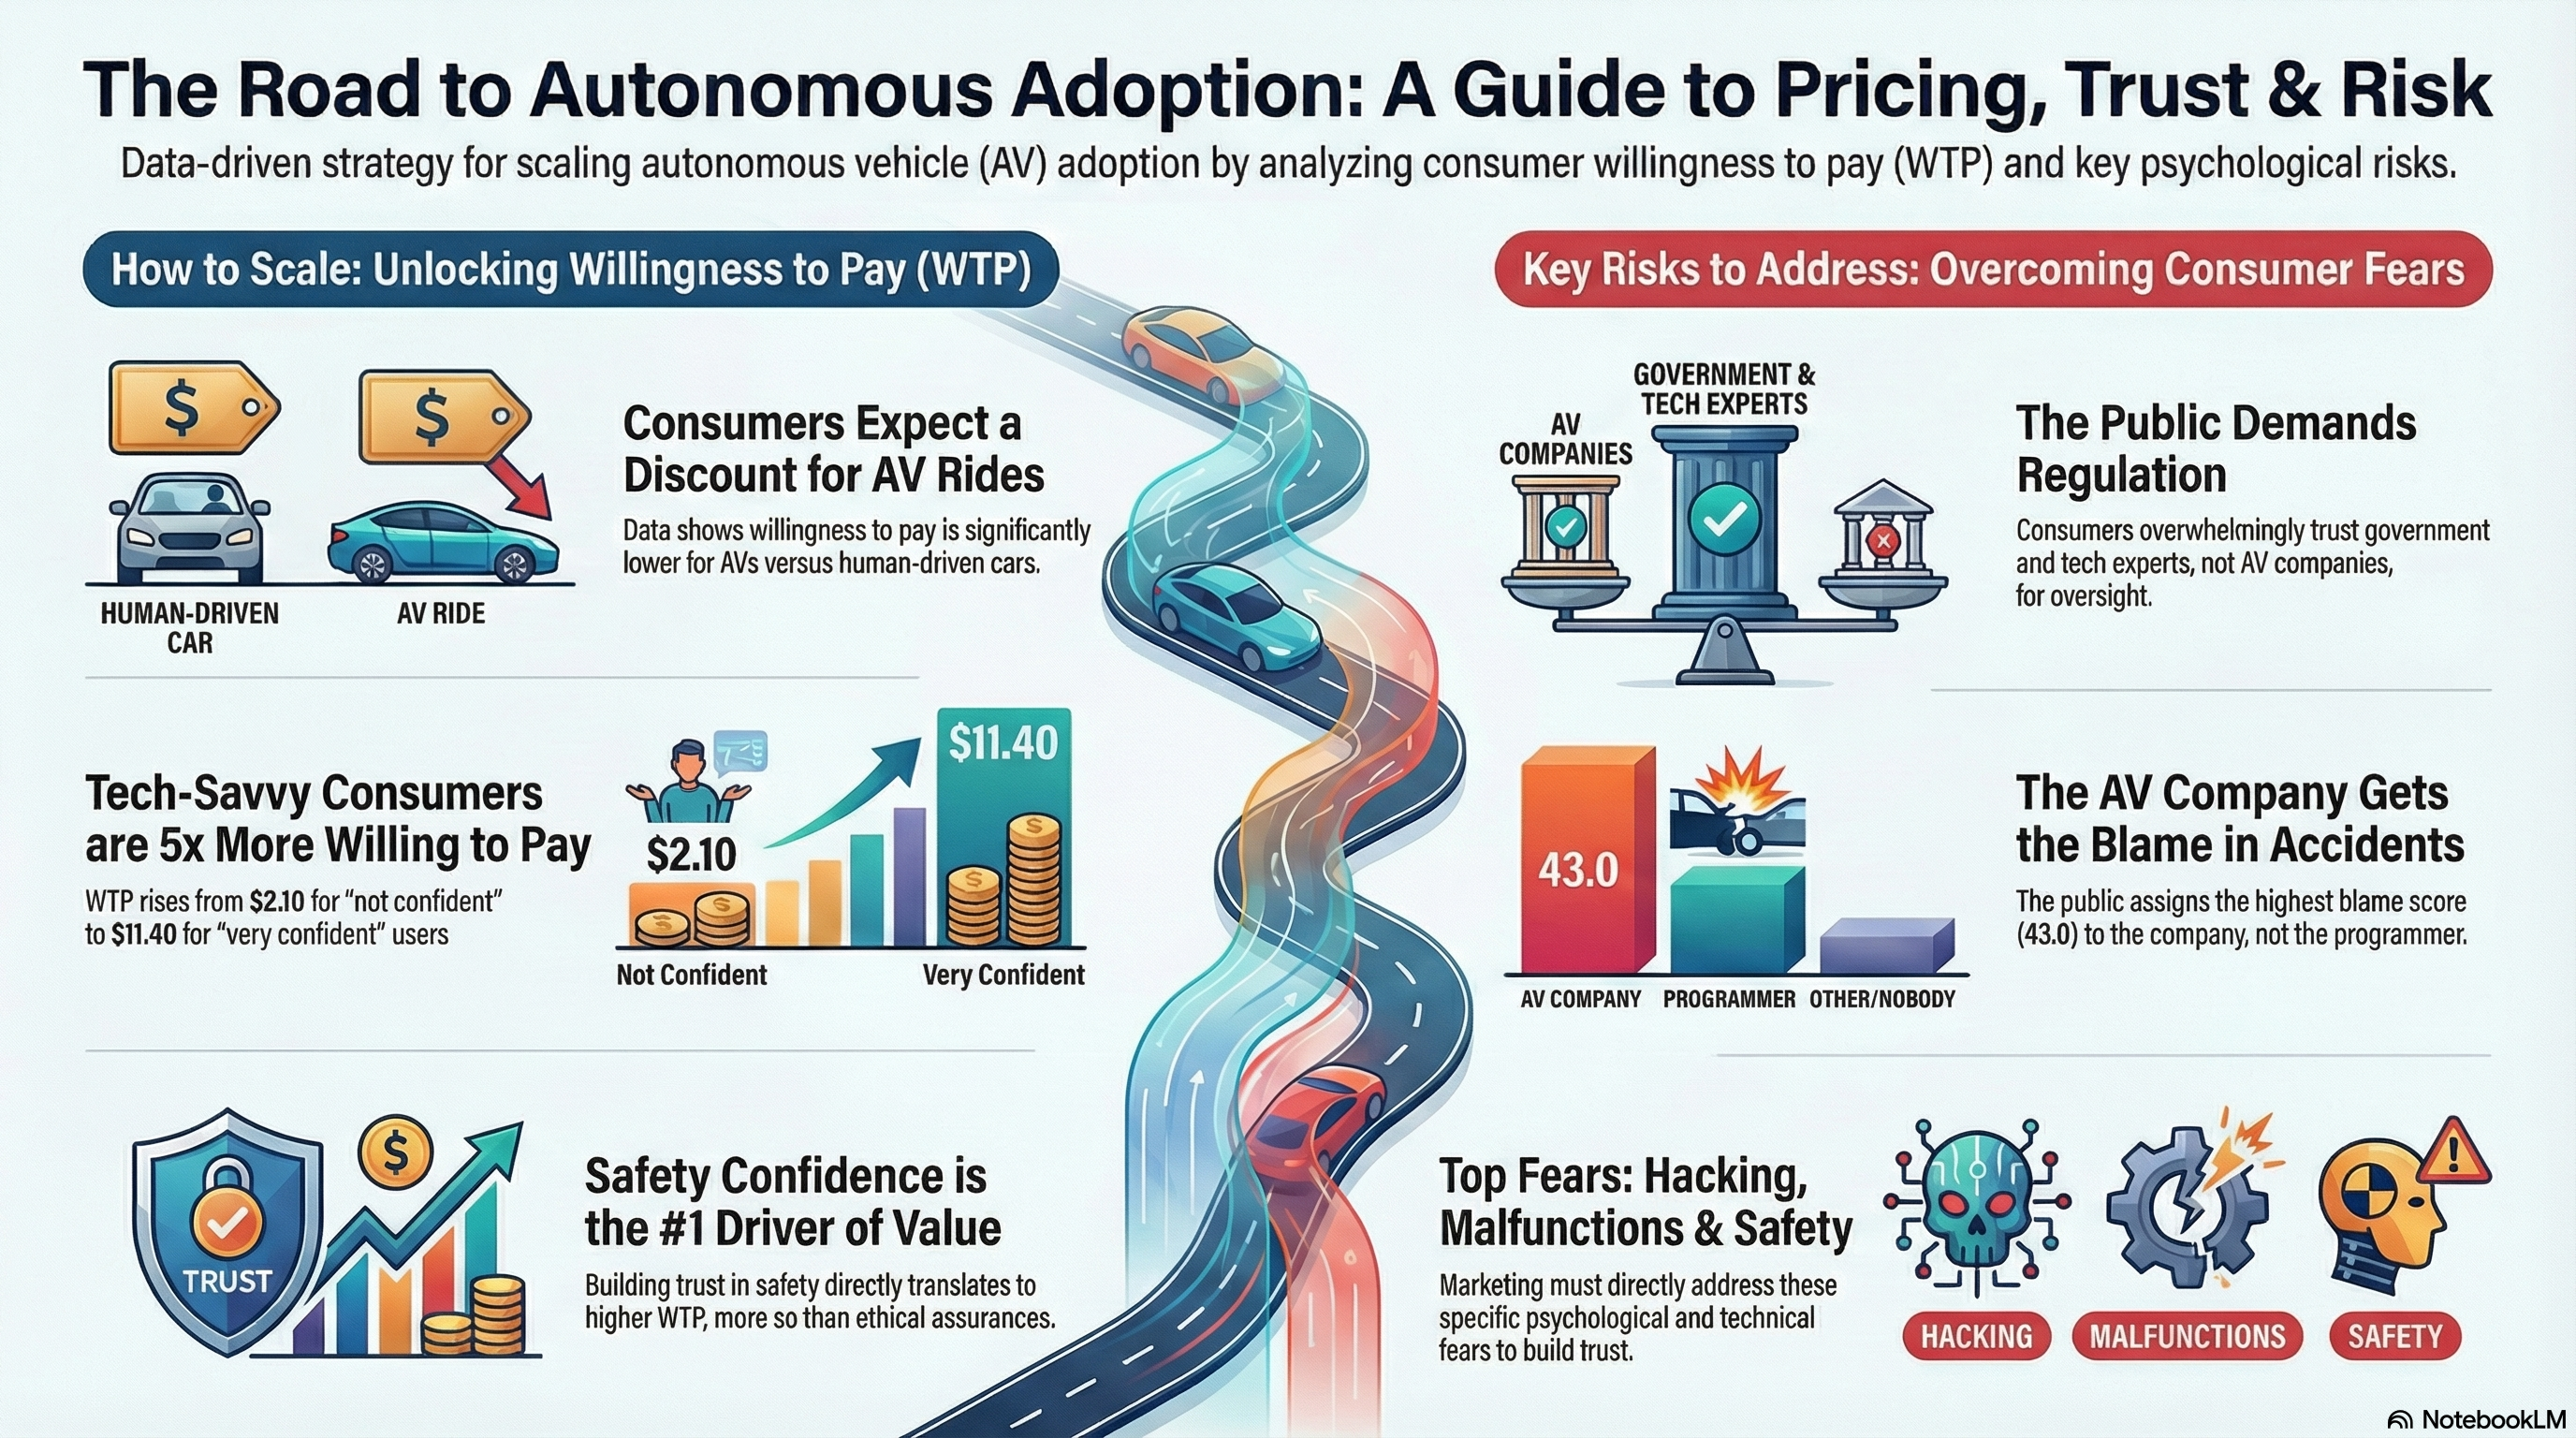
\includegraphics[width=1\linewidth,height=\textheight,keepaspectratio]{images/InfoGraphicOverview.png}
\end{center}

\subsection{Video Summary}\label{video-summary}

\bookmarksetup{startatroot}

\chapter{Reference}\label{reference}

\bookmarksetup{startatroot}

\chapter{Reference}\label{reference-1}

\begin{enumerate}
\def\labelenumi{\arabic{enumi}.}
\tightlist
\item
  R Core Team (2024). \emph{R: A language and environment for
  statistical computing}. R Foundation for Statistical Computing,
  Vienna, Austria. URL https://www.R-project.org/.
\item
  Wickham, H., Averick, M., Bryan, J., Chang, W., McGowan, L. D.,
  François, R., Grolemund, G., Hayes, A., Henry, L., Hester, J., Kuhn,
  M., Pedersen, T. L., Miller, E., Bache, S. M., Müller, K., Ooms, J.,
  Robinson, D., Seidel, D. P., Spinu, V., Takahashi, K., Vaughan, D.,
  Wilke, C., Woo, K., \& Yutani, H. (2019). \emph{Welcome to the
  tidyverse}. Journal of Open Source Software, 4(43), 1686.
  https://doi.org/10.21105/joss.01686.
\item
  Xie, Y., Allaire, J. J., \& Grolemund, G. (2018). \emph{R Markdown:
  The Definitive Guide}. Chapman and Hall/CRC.
  https://bookdown.org/yihui/rmarkdown.
\item
  Wickham, H. (2016). \emph{ggplot2: Elegant Graphics for Data
  Analysis}. Springer-Verlag New York. https://ggplot2.tidyverse.org.
\item
  Dowle, M., \& Srinivasan, A. (2024). \emph{data.table: Extension of
  \texttt{data.frame}}. R package version 1.14.8.
  https://CRAN.R-project.org/package=data.table.
\item
  Hester, J., Wickham, H., \& Francois, R. (2024). \emph{readr: Read
  Rectangular Text Data}. R package version 2.1.4.
  https://CRAN.R-project.org/package=readr.
\item
  Wickham, H., François, R., Henry, L., \& Müller, K. (2024).
  \emph{dplyr: A Grammar of Data Manipulation}. R package version 1.1.2.
  https://CRAN.R-project.org/package=dplyr.
\item
  Slowikowski, K. (2024). \emph{ggrepel: Automatically Position
  Non-Overlapping Text Labels with `ggplot2'}. R package version 0.9.4.
  https://CRAN.R-project.org/package=ggrepel.
\item
  Kassambara, A. (2024). \emph{ggpubr: `ggplot2' Based Publication Ready
  Plots}. R package version 0.6.4.
  https://CRAN.R-project.org/package=ggpubr.
\item
  Google Gemini 3. (2025). \emph{Google Gemini 3 Language Model}.
  https://ai.google.com/research/gemini.
\item
  Notebooklm by Google. (2025). \emph{NotebookLM: Your AI Research
  Notebook}. https://notebooklm.google.com/.
\end{enumerate}




\end{document}
